\documentclass[../root.tex]{subfiles}


\begin{document}
\chapter{
    Scalable Cooperative Transport of Cable-Suspended loads with UAVs using
    Distributed Trajectory Optimization
} \label{chap:distributed}
\chaptermark{Distributed Trajectory Optimization}
\lettrine{I}{n} this chapter we apply the methods from Chapter \ref{chap:altro} in a
distributed algorithm to solve the quadrotor team-lift problem. This
relatively simple approach to parallelization was an important starting
point for the later work detailed previously in Chapters \ref{chap:rslqr} and 
\ref{chap:mctrajop}. 
The content of this chapter was originally published in 
\cite{jackson_Scalable_2020}.

\section{Introduction}
Many robotic tasks can be accomplished by a single agent,
but often there are benefits to employing a team of robots. For example,
transporting a heavy load can be accomplished by deploying a single powerful,
expensive, and potentially dangerous aerial vehicle, or by deploying a group
of smaller aerial vehicles that cooperatively transport the load. The
potential benefits of a team approach, namely reduced cost, increased
versatility, safety, and deployability of the system, are important but come
at the cost of increased complexity. Motion planning for a single robot is
already a challenging task, and coordinating a group of agents to
cooperatively accomplish a task can be significantly more complicated due to
increased degrees of freedom, more constraints, and the requirement to reason
about the effects of distributed computation and communication.

\begin{figure}[t]
	\centering
	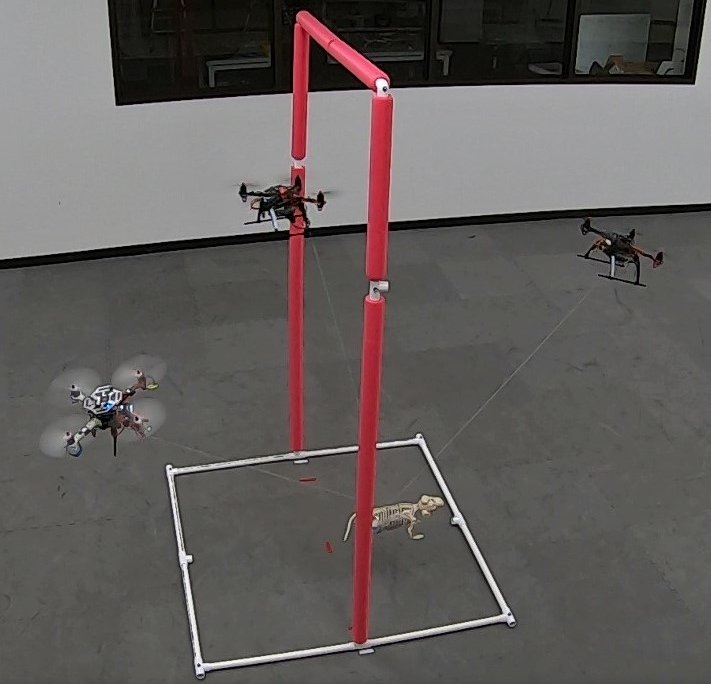
\includegraphics[width=6.5cm]{distributed/dogGate.jpg}
	\caption{Hardware experiment with a team of 3 quadrotors carrying a heavy
	load that a single quadrotor cannot lift. The team must reconfigure to
	proceed through the narrow doorway.}
	\label{fig:x0_hardware}
\end{figure}

Approaches for multi-agent motion planning range from decentralized methods
that consider local interactions of the agents to centralized methods that
globally coordinate a system of agents. The decentralized approach has many
advantages, such as robustness to agent removal or failure, scalability,
computational efficiency and, possibly, reduced communication requirements
among the network of agents. While decentralized approaches can achieve
useful and interesting global behavior 
\cite{cortes_Coverage_2004,krick_Stabilisation_2009,olfati-saber_Consensus_2004,
pimenta_Sensing_2008,vandenberg_Reciprocal_2008},
they have important limitations. Often, they are limited
to simple, homogeneous dynamics, such as single or double integrators. It is
also difficult to enforce constraints, either at the agent or the system
level.

Centralized approaches, in contrast, are able to reason about general
dynamics and constraints. However, they typically necessitate increased
computation and communication, and require solving large optimization
problems. Centralized methods are, therefore, typically run offline.
Additionally, since the optimization problems involved often exhibit cubic or
exponential scaling of computation time with the number of decision
variables, centralized approaches tend to scale poorly for systems with a
large number of agents. Both centralized and decentralized approaches have
been used in a large variety of fields, from controlling swarms of microscale
robots \cite{woern_Iswarm_2006}, to modeling human crowds \cite{bera_Realtime_2014},
to planning motion for teams of aerial vehicles
transporting heavy loads.

Aerial vehicles have been used to transport slung loads since at least the
1960s \cite{lancashire_Investigation_1966} for applications including:
delivering fire retardant to fight forest fires, carrying beams for civil
infrastructure projects, moving harvested trees, carrying military vehicles,
and transporting large animals. Today, quadrotors have become a standard
testbed for such aerial vehicle applications, and there is an extensive
literature on utilizing a single quadrotor to carry a slung load
\cite{sreenath_Geometric_2013,tang_Mixed_2015,decrousaz_Aggressive_2014,foehn_Fast_2017}.

Teams of quadrotors have also been explored, oftentimes making significant
simplifying assumptions. The most common simplification, and one also taken
in the current work, is to model the cables as massless rigid links
\cite{michael_Cooperative_2011,bernard_Autonomous_2011,tang_Aggressive_2018,lee_Geometric_2013,lee_Geometric_2014}
More recent approaches have relaxed this
assumption by modeling the system as a hybrid dynamical system and then
solving the problem as a mixed-integer program that takes nearly an hour to
solve \cite{tang_Mixed_2015}. While most assume a simple point mass for the
load, some also consider extensions to rigid bodies
\cite{michael_Cooperative_2011,lee_Geometric_2014}. 
A distributed controller for
a group of quadrotors rigidly attached to a load, assuming no communication
between agents \cite{wang_Cooperative_2018} has also been developed.

Beyond the suspended-load problem, collision-free trajectories for a swarm of
quadrotors can be calculated using sequential convex programming, but the
computational complexity scales exponentialy with the number of agents
\cite{augugliaro_Generation_2012}. Other notable examples of coordinated teams
of quadrotors include throwing and catching a ball with quadrotors connected
by a net \cite{ritz_Cooperative_2012}, performing a treasure hunt
\cite{spurny_Cooperative_2019}, and manipulating flexible payloads
\cite{ritz_Carrying_2013}. Distributed approaches for motion planning have been
proposed using alternating direction method of multipliers (ADMM) and mixed
integer programs
\cite{vanparys_Online_2016,inalhan_Decentralized_2002,kuwata_Cooperative_2010,
park_Distributed_2019},
% \cite{van2016online,inalhan2002decentralized,kuwata2010cooperative,park2019distributed},
but they utilize simplified dynamics or constraints, and don't consider
interaction between agents (e.g., forces). 

In this work, we present a scalable distributed approach for obtaining
a solution to the centralized ``batch'' motion-planning
problem for a team of quadrotors carrying a cable-suspended load and
demonstrate the algorithm in hardware (Fig. \ref{fig:x0_hardware}).
This approach combines the generality of centralized methods, while
approaching near real-time performance that would be impossible without
distributed, parallel computation. We formulate a trajectory optimization
problem and consider the nonlinear rigid body
dynamics of the quadrotors and non-convex collision and obstacle
avoidance constraints. We use the trajectory
optimization solver ALTRO \cite{howell_ALTRO_2019} to find the state
and control trajectories for the system of agents. To make the problem
scalable in the number of agents, we take an intuitive approach of
decomposing the problem by agent and solving the resulting subproblems in
parallel. The result is a substantial
reduction in solution time and superior scaling as the number of agents is
increased. The novelty of this approach lies in the use of a
trajectory optimization solver (in our case, ALTRO) to solve a sequence of
smaller constrained problems, that include optimizing interactions (i.e.,
forces) between agents, instead of solving a single large trajectory
optimization problem.

The remainder of this paper is organized as follows:  Section \ref{batch_problem}
formulates the cable-suspended-load problem as a trajectory optimization
problem. Section \ref{dist_batch_problem} presents a decomposition scheme and
an algorithm for solving the batch problem in parallel among agents. Section
\ref{sim_results} contains simulation results and Section
\ref{hardware_results} contains details of the hardware experiments. Finally,
we conclude with a discussion of the algorithm and results in Section
\ref{discussion}.

\section{Batch Problem}\label{batch_problem}
We formulate a trajectory optimization problem for the team cable-suspended
load problem with $L$ quadrotors attached to a point-mass load. The
suspension cables are assumed to pass through the center of mass of each
quadrotor, and are modeled as massless rigid links. The dynamics model
formulation of the system is critical for
achieving good performance using trajectory optimization,
and is described in detail in Section \ref{sec:dynamics}. Section
\ref{sec:batch_problem} then describes the optimization problem.

\subsection{Dynamics} \label{sec:dynamics}
\subsubsection{Quadrotor Model with Quaternions} 
The quadrotor dynamics presented in \cite{mellinger_Trajectory_2012} are
modified to use quaternions for angular representation and incorporate the
force generated by a suspension cable:

\begin{equation} \label{eq:quad_dynamics}
\begin{aligned}
\dot{x} &=
\begin{bmatrix}
\dot{r} \\ \dot{q} \\ \dot{v} \\ \dot{\omega}
\end{bmatrix} 
= 
\begin{bmatrix}
v \\ 
\frac{1}{2} q \otimes \hat{\omega} \\
g + \frac{1}{m^i} (R(q)F(u) + F_c(u_5,x,x^\ell)) \\ 
J^{-1}(\tau(u) - \omega \times J \omega)
\end{bmatrix} \\
&= f(x,u; x^\ell)
\end{aligned}
\end{equation}
where $r \in \mathbb{R}^3$ is the position, $q$ is a unit quaternion, $R(q)
\in \mathbb{SO}(3)$ is a quaternion-dependent rotation matrix from body frame
to world frame, $v \in \mathbb{R}^3$ is the linear velocity in the world
frame, $\omega \in \mathbb{R}^3$ is the angular velocity in the body frame,
$x \in \mathbb{R}^{13}$ is the state vector, $u \in \mathbb{R}^5$ is the
control vector with the last component being the magnitude of the cable
force, $x^\ell \in \mathbb{R}^6$ is the state vector of the load (defined
below), $g \in \mathbb{R}^3$ is the gravity vector, and $m^i \in \mathbb{R}$
is the mass of the $i$-th quadrotor, $J \in \mathbb{S}^3$ is the moment of
inertia tensor, $q_2 \otimes q_1 $ denotes quaternion multiplication,
and $\hat{\omega}$ denotes a quaternion with zero scalar part, and $\omega$
vector part. Quaternions are used to easily allow for large angular
displacements and extensions to more aggressive maneuvers. The forces and
torques $F,\, \tau \in \mathbb{R}^3$ in the body frame are
\begin{equation}
	F(u) = \begin{bmatrix} 0 \\ 0 \\ k_f(u_1 + u_2 + u_3 + u_4) \end{bmatrix}
\end{equation}
\begin{equation}
\tau(u) = \begin{bmatrix} 
	k_f d_\text{motor} (u_2 - u_4) \\ 
	k_f d_\text{motor} (u_3 - u_1) \\ 
	k_m (u_1 - u_2 + u_3 - u_4)
\end{bmatrix}
\end{equation}
where $k_f$, $k_m$ are motor constants, $d_\text{motor}$ is the distance
between motors, and $u_{1:4}$ are motor thrusts. Forces from the cables,
modeled in the world frame, are calculated as:
\begin{equation}
F_c(\gamma,x,x^\ell) = \gamma \frac{r^\ell - r}{\norm{r^\ell - r}}_2,
\end{equation}
where $\gamma \in \mathbb{R}$ ($u_5$ for each quadrotor) is the magnitude of
the tension in the cable and $r^\ell$ is the three-dimensional position of
the load.

\subsubsection{Load}
The dynamics of a load being transported by $L$ quadrotors are:
\begin{equation} \label{eq:load_dynamics}
\begin{aligned}
\dot{x}^\ell &= 
\begin{bmatrix}
\dot{r}^\ell \\ \dot{v}^\ell 
\end{bmatrix} =
\begin{bmatrix}
v^\ell \\ g + \frac{1}{m^\ell} F^\ell(x^{\ell},u^{\ell}, x^1,..., x^L)
\end{bmatrix} \\
&= f^\ell(x^\ell, u^\ell; x^1, \dots, x^L)
\end{aligned}
\end{equation}
where $r^\ell$ is the three-dimensional position, $v^\ell$ is the linear
velocity in the world frame, $m^\ell$ is the mass of the load, $x^\ell \in
\mathbb{R}^6$ is the state vector, $u^\ell \in \mathbb{R}^L$ is the force
acting on the load (not a direct control input), $x^i$ is the state vector of
quadrotor $i$, and
\begin{equation}
F^\ell(x^{\ell},u^\ell, x^1, ..., x^L) = - \sum_{i=1}^L F_c(u^\ell_i, x^i, x^\ell).
\end{equation}

\subsection{Optimization Problem} \label{sec:batch_problem}
The batch problem is formulated by concatenating the states and controls of
$L$ quadrotors and the load:
\begin{equation}
\bar{x} \in \mathbb{R}^{13L+6}= \begin{bmatrix} x^1 \\ \vdots \\ x^L \\ x^\ell \end{bmatrix}, \quad
\bar{u} \in \mathbb{R}^{5L+L} = \begin{bmatrix} u^1 \\  \vdots \\ u^L \\ u^\ell \end{bmatrix}.
\end{equation}
where $\mathcal{I}_L = \{1,\dots,L\}$ are the indices of the quadrotors and
$\mathcal{I}_A = \{1,\dots,L,\ell\}$ are the indices of all the agents
(including the load). We can pose the team cable-suspended-load problem as a
single trajectory optimization problem:
\begin{mini!}[3]
	{\mathbf{X},\mathbf{U}}{ J^{\ell}(X^\ell,U^\ell) + \sum_{i=1}^L J^i(X^i,U^i) }{}{} \label{opt:quad_lift}
	\addConstraint{x_{k+1}^i }{= f_k^i (x_k^i,u_k^i, \Delta t;x_k^\ell),}
	{\forall i \in \mathcal{I}_L}
	\label{con:dynamics}
	\addConstraint{x_{k+1}^\ell }
	{= f_k^{\ell}(x_k^\ell,u_k^\ell,\Delta t;x_k^1,\dots,x_k^L)}
	\label{con:load_dynamics}
	\addConstraint{x_0^i }{= x(0)^i,}
	{\forall i \in \mathcal{I}_A}
	\label{con:initial_conditions}
	\addConstraint{x_N^\ell }{= x(t_f)^\ell}{}
	\label{con:final_conditions}
	\addConstraint{r_{\text{min}}^i \leq r_k^i }{\leq r_{\text{max}}^i,}
	{\forall i \in \mathcal{I}_A}
	\label{con:workspace}
	\addConstraint{0 \leq (u_k^i)_j }{\leq u_{\text{max}}^i, }
	{\forall i \in \mathcal{I}_L, j \in \{1,\dots,4\}}
	\label{con:max_thrust}
	\addConstraint{ u_k^\ell }{\geq 0 }{} \label{con:taut}
	\addConstraint{(u_k^i)_5 }{= (u_k^\ell)_i, }
	{\forall i \in \mathcal{I}_L}
	\label{con:equal_force}
	\addConstraint{\norm{r_k^i - r_k^\ell}_2 }{= d_{\text{cable}},}
	{\forall i \in \mathcal{I}_L}
	\label{con:length}
	\addConstraint{2d_{\text{quad}} -\norm{p_k^i - p_k^j}_2 }{\leq 0,}
	{\forall i,j \in \mathcal{I}_L, i \neq j}
	\label{con:collision}
	\addConstraint{d_{\text{quad}} + d_{\text{obs}} - \norm{p_k^i - p_{\text{obs}}^j}_2 }{\leq 0,}
	{\forall i \in \mathcal{I}_L, \forall j}
	\label{con:quad_obs}
	\addConstraint{d_{\text{load}} + d_{\text{obs}} - \norm{p_k^\ell - p_{\text{obs}}^j}_2 }{\leq 0,}
	{\forall j}
	\label{con:load_obs},
\end{mini!} 					
where $X = [x_0,\dots,x_N]$ is a state trajectory of length $N$, $U =
[u_0,\dots,u_{N-1}]$ is a control trajectory of length $N-1$, $\mathbf{X} =
[X^1,\dots,X^L,X^{\ell}]\, \text{and}\, \mathbf{U} =
[U^1,\dots,U^L,U^{\ell}]$ are sets of trajectories for the system, $p^i \in
\mathbb{R}^2$ is the two-dimensional position of the quadrotor or load
(discarding height), $x(0)$ and $x(t_f)$ are initial and final
conditions, $d$ is a scalar dimension (e.g., quadrotor radius), $\Delta t$
is the time step duration, and all constraints apply at each time steps $k$.

The constraints are, from top to bottom: discrete quadrotor dynamics
\eqref{con:dynamics} from \eqref{eq:quad_dynamics}, discrete load dynamics
\eqref{con:load_dynamics} from \eqref{eq:load_dynamics}, initial conditions
\eqref{con:initial_conditions}, final condition for the load
\eqref{con:final_conditions}, workspace constraints (i.e. floor and ceiling
constraints) \eqref{con:workspace}, quadrotor motor constraints
\eqref{con:max_thrust}, positive cable tension \eqref{con:taut}, equal
tension force on quadrotor and load \eqref{con:equal_force}, cable length
\eqref{con:length}, collision avoidance \eqref{con:collision}, and obstacle
avoidance for the quadrotors \eqref{con:quad_obs} and load
\eqref{con:load_obs}. The obstacles are modeled as cylinders of
infinite height, which reduces collision checking to a plane. These simple
constraints can be combined to form narrow doorways or slots and enables
fast, analytical collision checking. The self-collision constraints
also model the quadrotors as cylinders of infinite height to
help prevent unmodeled prop wash effects from disturbing the system. The
objective for each agent was a quadratic cost, having the form: $(x_k -
x_{\text{ref}})^T Q_k (x_k - x_{\text{ref}})$ and $(u_k - u_{\text{ref}})^T
R_k (u_k - u_{\text{ref}})$ for the states and controls, respectively, at
each time step $k$.

We found it beneficial to both initialize the solver and include in the
objective state and control references: $x_{\text{ref}}$, $u_{\text{ref}}$,
based on trim conditions that produce static hovering of the system. These
conditions were found using trajectory optimization by setting the initial
and final positions and velocities of the system to be the same. Large costs
were used for all states except the orientation, which had a relatively small
cost. Solving this problem, the system naturally finds an equilibrium state
where the quadrotors ``lean away'' from the load in order to create thrust in
a direction that compensates for the tension in the cable (this behavior can
be seen in Fig. \ref{fig:x0_hardware}). These quadrotor orientations are then
used for the initial and final orientations and the trim controls are used as
reference controls. Regularizing the control values to these trim controls,
rather than to zero, had a significant effect on the convergence of the
optimization. This hover condition was also used as the initial control
trajectory provided to ALTRO.

\section{Distributed Formulation} \label{dist_batch_problem}
We present a scalable approach for solving \eqref{opt:quad_lift} by
decomposing the problem by quadrotor. Of the given constraints, only the
collision avoidance constraint \eqref{con:collision} directly couples the
states of the quadrotors (i.e. only the collision avoidance
constraints are functions of the states of different quadrotors). The
quadrotors' dynamics are only indirectly coupled (through the load) via the
cable constraints \eqref{con:equal_force} and \eqref{con:length}. The
objective, by design, is separable by agent, i.e. there is no cost
coupling between the state and controls of the quadrotors or the quadrotors
and load.

From these observations, a decomposition is quite apparent: solve a
trajectory optimization problem for each quadrotor independently, treating
all other quadrotor and load trajectories as static.
After each quadrotor has optimized independently, the
updated trajectories are collected and used to optimize the load trajectory.
The updated load trajectory, along with the updated quadrotor trajectories,
are then communicated to each quadrotor and the process is repeated.

While this update for the load trajectory can be considered a
consensus update, it is distinct from approaches like ADMM that perform
primal updates over agents followed by a collective dual update. In our
approach, each agent performs primal and dual updates until convergence
before communicating. In practice, we found this approach to converge faster
and more reliably. Our procedure is summarized in Algorithm
\ref{alg:dist_traj_opt}.

\begin{algorithm}[h]
	\begin{algorithmic}[1]
		\caption{Distributed Trajectory Optimization} \label{alg:dist_traj_opt}
		\Function{dist-traj-opt}{$\textbf{X}_0, \textbf{U}_0, \text{tol.}$}
		\State $\tilde{\textbf{X}} \leftarrow \textbf{X}_0, \, \tilde{\textbf{U}} \leftarrow \textbf{U}_0 $
		\While{$\Call{max-violation}{\tilde{\textbf{X}},\tilde{\textbf{U}}} > \text{tol.}$}
		\For{$i = 1,\dots,L$ }{\, in parallel}
		\State $X^i, U^i \leftarrow \Call{solve-quad}{X^i,U^i; \tilde{\textbf{X}},\tilde{\textbf{U}}}$
		\State send $X^i, U^i$ to central agent
		\EndFor
		\State $X^{\ell}, U^{\ell} \leftarrow \Call{solve-load}{X^\ell,U^\ell; \tilde{\textbf{X}},\tilde{\textbf{U}}}$
		\State send $\tilde{\textbf{X}},\tilde{\textbf{U}}$ to all agents
		\EndWhile \\
		\Return $\tilde{\textbf{X}},\tilde{\textbf{U}}$
		\EndFunction
	\end{algorithmic}
\end{algorithm}
\noindent The ``central'' agent (the one that computes the load trajectory)
is, in practice, randomly assigned before the solve to one of the quadrotors,
and is computed in a separate process with a separate memory space.

As with most nonlinear optimization algorithms, the performance of our
algorithm improves dramatically with a good initial guess. We designed our
guess by solving an initial set of trajectory optimization problems for each
quadrotor and the load separately, without any of the system-level
constraints (i.e., self-collision \eqref{con:collision} or cable constraints
\eqref{con:equal_force} and \eqref{con:length}). Since these problems are
completely de-coupled, they can be solved in parallel. Getting these initial
trajectories to be sufficiently close to the final solution was key in
getting the fast convergence demonstrated in the results that follow. The
time to solve these initial trajectory optimization problems is included in
the overall solution time. These optimizations were initialized with
the same trim conditions given to the batch problem, described previously.
However, for these initial optimization problems, the initial control and
control reference for the cable tension was set to zero, since the cable
constraints weren't considered during these problems. This resulted in
slightly different initializations for the batch and distributed algorithms.

\section{Simulations} \label{sim_results}

\subsection{Scenarios}
Three scenarios using the batch problem formulation are
considered: 1) point-to-point transfer of a load using $L$ quadrotors (see
Fig. \ref{Lsystem}), 2) a load transfer through a narrow slot,
followed by a narrow doorway, which requires the quadrotors to spread apart
and then gather together (see Fig. \ref{fig:slot_scenario}), and
3) a load transfer through a narrow doorway using 3 quadrotors
(see Fig. \ref{composite}). All scenarios solve a 10 s
trajectory. We assume perfect knowledge of the obstacles.

In the first and second scenarios, the stage costs were identical for
all time steps. The costs for the second and third scenarios were
identical; however, in the third scenario, the cost was
altered at the middle time step $k_m = (N-1)/2$ to encourage the quadrotors
to ``line up'' when passing through the door. This stage cost simply placed a
high cost (about equal in magnitude to the cost at the terminal time step)
for deviations from an intermediate configuration for passing through the
doorway.
%	\begin{equation}
%		\Delta t \Big((r_k^i - r_m^i)^T W_m (r_k^i - r_m^i) +(u_k^i - u_{m_r}^i)^T R_k (u_k^i - u_{m_r}^i)\Big),
%	\end{equation}
%	where $r_m^i$ is the desired position of agent $i$ as it passes through the door, $W_m \in \mathbb{S}_{+}^3$ has weights about equal in magnitude to those in $W_N$, and $u_{m_r}^i$ is a control reference for this position. 
The desired positions were calculated directly from the initial position of
the load and the location of the center of the door. The load was assumed to
be at the center of the door, at the same height it started. The quadrotors
are then evenly distributed on an arc of $\alpha$ degrees. This encourages
the quadrotors to ``fan'' out around the load, see Fig.
\ref{fig:x0_hardware}). 

The dimensions of the quadrotor, load cables, and doorway were based
on the actual values for the hardware experiment (see Section
\ref{hardware_results}). In simulation, the slot and doorways are modeled
using horizontally and vertically oriented cylinder obstacle constraints. The
doorway in Fig. \ref{composite} was constructed from two cylinders 2 m apart
with a radius of 0.5 m, 0.6 m smaller than the actual doorway (1.0 m vs 1.6
m). The slot scenario is similarly dimensioned. To encourage the quadrotors
to get in position before reaching the door, we made the doorway artificially
``deep'' by adding a second set of cylinders. The width of the quadrotor was
set to 0.55 m. This scenario is challenging since, although a single
quadrotor can fit through the doorway easily, two cannot. The quadrotors must
coordinate a way to carry the load through the doorway while passing through
one at a time.


\subsection{Results}
We define two methods for solving (\ref{opt:quad_lift}):

\begin{itemize}
	\item Batch - solve directly
	\item Parallel - solve using Algorithm \ref{alg:dist_traj_opt} with multiple cores on the same or distributed machines
\end{itemize}

All trajectory optimization sub-problems were solved using ALTRO to a maximum
constraint violation of 1e{-}3 and performed either on a desktop computer
with an AMD Ryzen Threadripper 2950x processor and 16GB RAM or an ODROID-XU4
microcomputer with a 32-bit Samsung Exynos5 Octa ARM Cortex-A15 2Ghz
processor and 2GB of RAM onboard the quadrotors. Algorithm
\ref{alg:dist_traj_opt} is implemented in the Julia programming language,
 uses the ALTRO trajectory optimization solver
\cite{howell_ALTRO_2019}, and leverages the language's convenient methods for
working with distributed computation. The solver hyper-parameters were tuned
to each algorithm (batch vs. distributed) but kept the same across all
scenarios.

Fig. \ref{fig:n_lift} contains the timing results for the first scenario with
$L$ ranging from 3 to 15 quadrotors, clearly demonstrating the scalability of
Algorithm \ref{alg:dist_traj_opt} compared to explicitly solving the batch
problem (\ref{opt:quad_lift}).

\begin{figure}[t]
	\centering
	\minipage{2.85cm}
	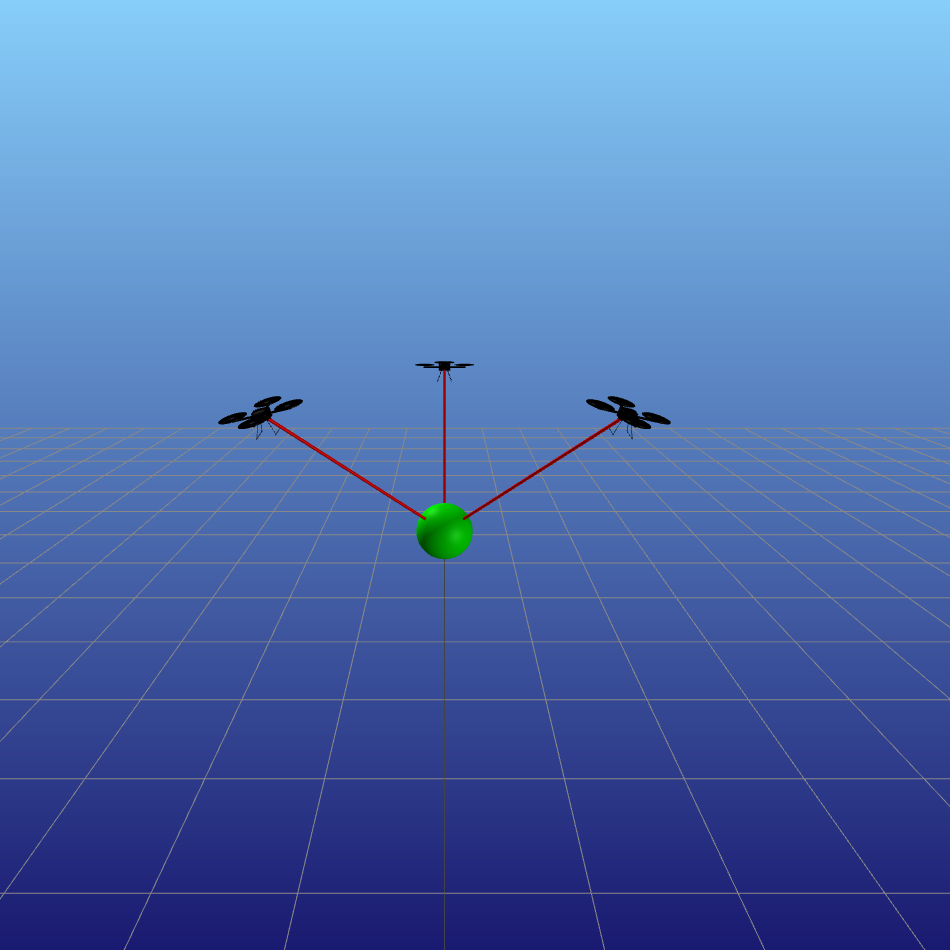
\includegraphics[width=2.75cm]{distributed/3quad_crop.png}
	\endminipage
	\minipage{2.85cm}
	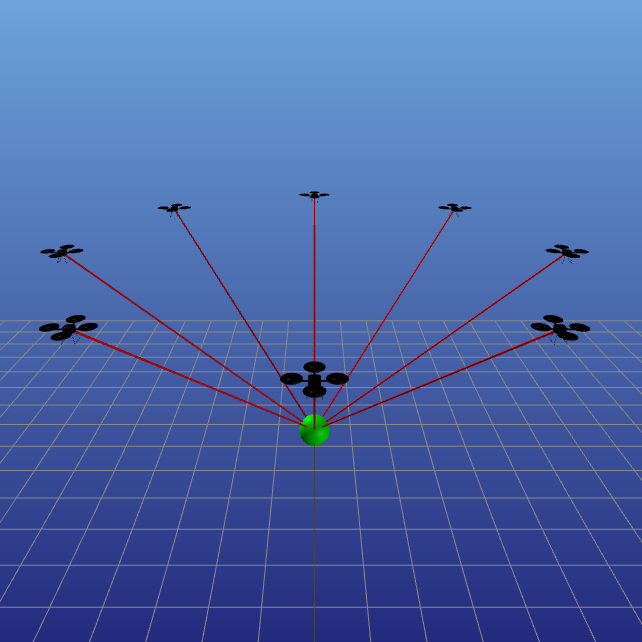
\includegraphics[width=2.75cm]{distributed/8_quad_crop.png}
	\endminipage
	\minipage{2.85cm}%
	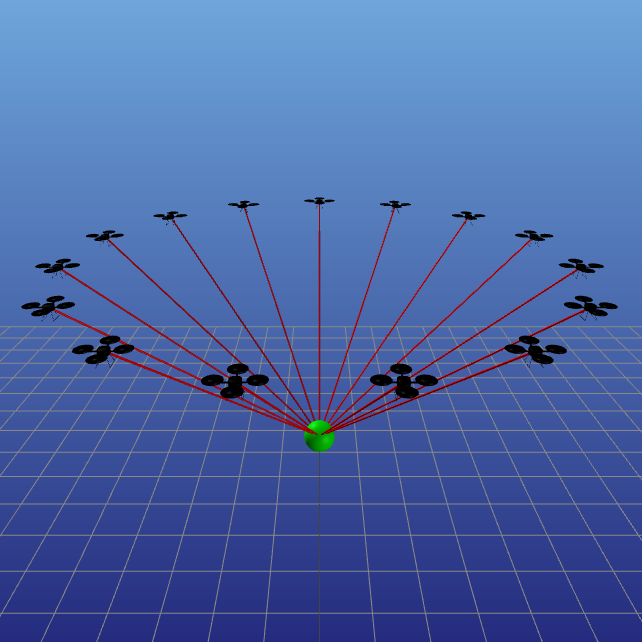
\includegraphics[width=2.75cm]{distributed/15_quad_crop.png}
	\endminipage
	\caption{Simulation of teams with 3, 8, and 15 quadrotors (left, center,
	right) in final configuration after a point-to-point load transfer. To
	maintain the final system configuration, quadrotors orient to produce
	thrust that maintains hover despite a force resulting from the load.}
	\label{Lsystem}
\end{figure}

\begin{figure}[t]
	\centering
	\includegraphics[width=\columnwidth,height=4.25cm]{distributed/L_lift.tikz}
	\caption{Timing result comparing batch and parallel algorithms for a
	point-to-point load transfer using $L$ quadrotors. The parallel algorithm
	scales favorably compared to the batch approach as the number of
	quadrotors is increased.}
	\label{fig:n_lift}
\end{figure}

When solving the second scenario, the batch version took 4.0 seconds
to solve, whereas the distributed version took only 2.0 seconds. To test
sensitivity of the algorithm to initial conditions, we varied the x position
by $\pm 1.5$m in the $x$ and $y$ direction ($+x$ is closer to the goal, and
$+z$ is vertical). The distributed version could solve problems within $\pm
0.5$m in $x$ and $\pm 1.5$m in $y$. The batch version solved problems within
$\pm 1.5$m in $x$ and $\pm 1.5$m in $y$. The batch version can handle a
larger set of initial conditions since it jointly optimizes all of the
trajectories, so will naturally be more robust.

\begin{figure}
	\centering
	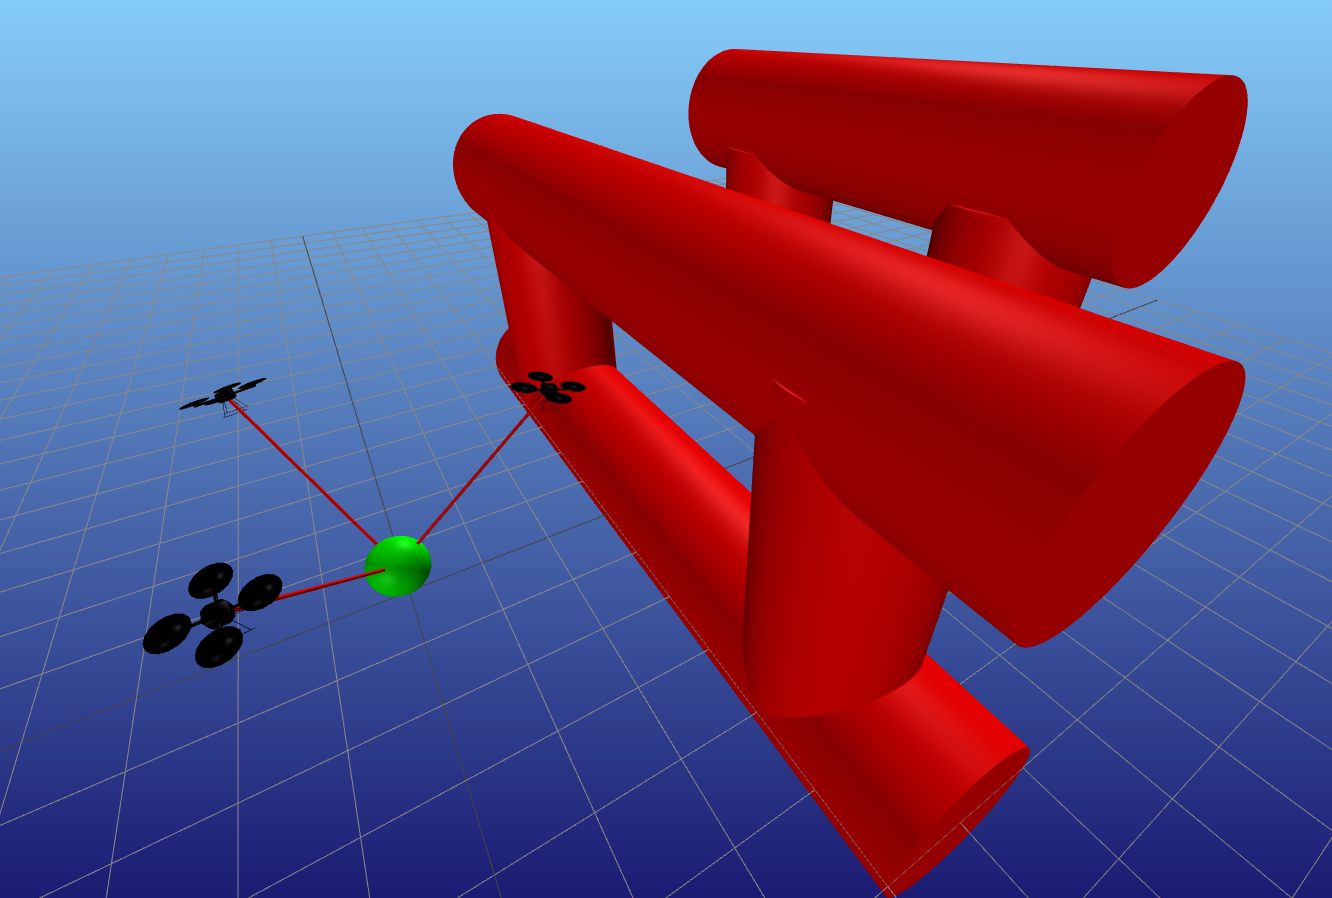
\includegraphics[width=0.7\columnwidth]{distributed/slot_scenario.png}
	\caption{Slot scenario. The quadrotors have to automatically
	reconfigure to pass through a narrow horizontal slot, followed by a
	narrow doorway.}
	\label{fig:slot_scenario}
\end{figure}

A sequence of frames from the doorway scenario is presented in Fig.
\ref{composite}, and the timing results for this scenario are included in
Table \ref{tab:door_timing}. The last row in the table was performed on the 3
ODROID-XU4 computers onboard the quadrotors used in the hardware
demonstration. One of the quadrotors was used as the ``central'' agent, which
used a separate core for solving the load problem. Communication between the
computers was performed over WiFi. The cost and constraint convergence
is compared in Figures \ref{fig:cost_convergence} and
\ref{fig:constraint_convergence}, respectively. The cost and constraint
values for the parallel solve were calculated by concatenating the current
values for the quadrotor and load trajectories. The distributed method starts
with a slightly higher initial cost and constraint violation since the
initial control trajectories assume zero force in the cable (since the
initial ``presolve'' neglects these constraints), whereas the the initial
guess for the batch method guesses the force from the trim conditions. Both
methods achieve the same constraint satisfaction, but the
distributed version achieves a slightly lower cost of
3.6 versus 4.6 for the
batch version. While the resulting trajectories
are similar, the distributed version results in a seemingly ``smoother''
trajectory, likely resulting from the guess provided by the ``presolve''
phase. The implementation and all simulation results are
available at:
\url{https://github.com/RoboticExplorationLab/TrajectoryOptimization.jl/tree/distributed_team_lift}

\begin{figure*}[t]
	\centering
	\begin{subfigure}{0.485\textwidth}
		\includegraphics[width=\columnwidth,height=4.25cm]{distributed/cost_convergence.tikz}
		\caption{Cost convergence}
		\label{fig:cost_convergence}
	\end{subfigure}
	~
	\begin{subfigure}{0.485\textwidth}
		\includegraphics[width=\columnwidth,height=4.25cm]{distributed/constraint_convergence.tikz}
		\caption{Constraint convergence}
		\label{fig:constraint_convergence}
	\end{subfigure}
	\caption{Convergence comparison of covergence of the cost function (a)
	and constraint violation (b) for the batch and distributed solves. The
	distributed solve is broken into three phases: 1) Presolve, where an
	initial trajectory for each agent is obtained by solving each problem
	independently, 2) Quads, where each quadrotor solves it's own problem in
	parallel, and 3) Load, where the trajectory for the load is solved using
	the updated quadrotor trajectories.}
\end{figure*}

\begin{figure}[t]
	\centering
	\minipage{.19\textwidth}
	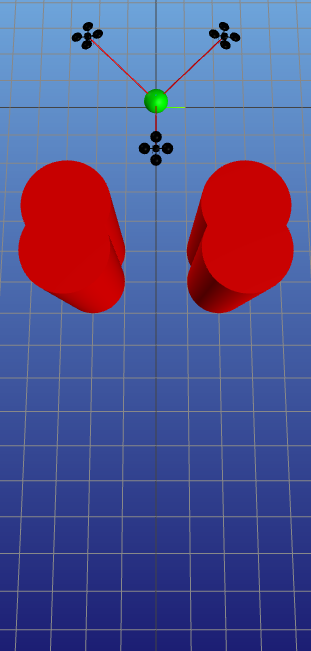
\includegraphics[width=.9\textwidth]{distributed/frame1_crop.png}
	\endminipage
	\minipage{.19\textwidth}
	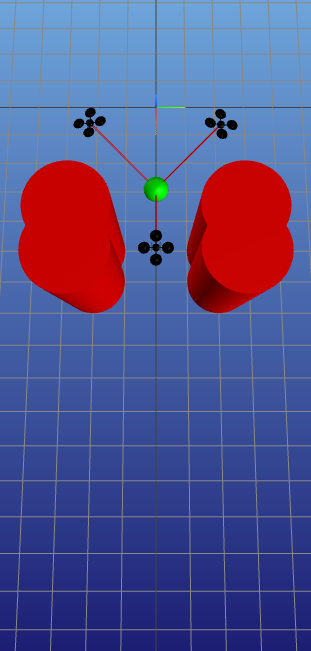
\includegraphics[width=.9\textwidth]{distributed/frame2_crop.png}
	\endminipage
	\minipage{.19\textwidth}%
	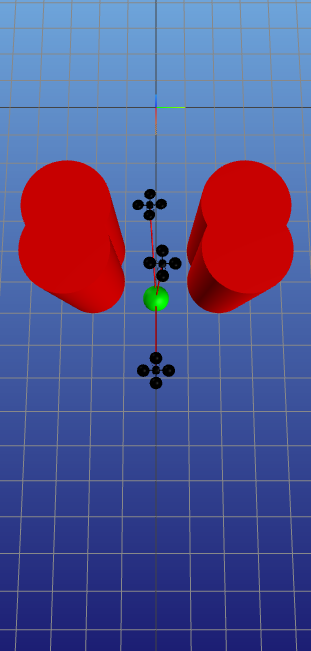
\includegraphics[width=.9\textwidth]{distributed/frame3_crop.png}
	\endminipage
	\minipage{.19\textwidth}%
	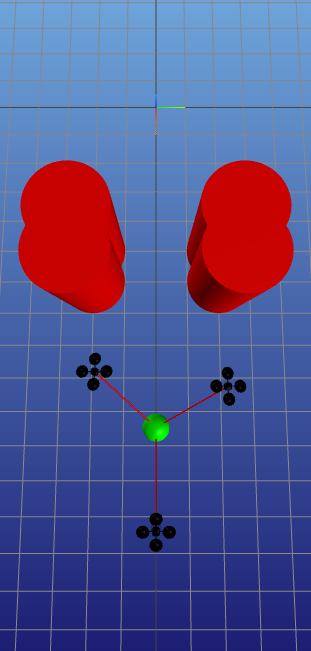
\includegraphics[width=.9\textwidth]{distributed/frame4_crop.png}
	\endminipage
	\minipage{.19\textwidth}%
	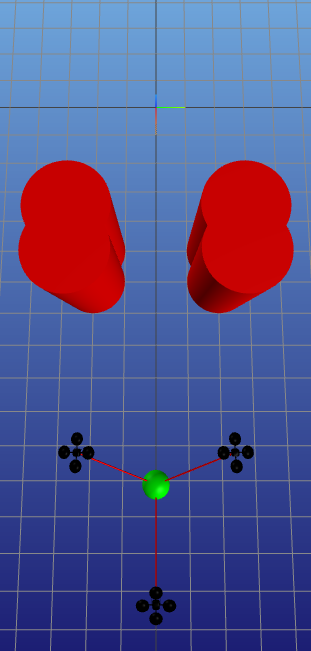
\includegraphics[width=.9\textwidth]{distributed/frame5_crop.png}
	\endminipage
	\caption{Simulation results of a team with 3 quadrotors transporting a
	load, that a single agent cannot lift, through a doorway during a 10 s
	trajectory. The system reconfigures to travel through the doorway and is
	shown at time instances t = 0.0, 2.4, 5.0, 7.6 10.0 s (left to right).}
	\label{composite}
\end{figure}

\begin{table}
	\centering
	\caption{Runtime performance: Doorway Scenario}
	\begin{tabular}{llll}
		\toprule
		\textbf{Computer} &
		\specialcellbold{Batch} &
		\specialcellbold{Parallel} \\
		\midrule
		Desktop & 3.6 s  & 0.8 s \\
		1 Quadrotor & 28.7 s & 5.4 s \\
		3 Quadrotors & - &  5.7 s \\
		\toprule
	\end{tabular}
	\label{tab:door_timing}
\end{table}

\section{Hardware Results}\label{hardware_results}

Hardware experiments were conducted with three custom-built quadrotor aerial
robots based on the F330 frame \cite{wang_Game_2019} in a 16.5 m $\times$ 6.5 m
$\times$ 2.7 m motion capture room. Each quadrotor ($m^i \approx$ 1 kg) was
equipped with a Pixfalcon, an open-source flight controller board, along with
the PX4 open-source autopilot software (v1.7.3) to manage low-level control
and real-time state estimation. Furthermore, each quadrotor used an
ODROID-XU4 for high-level trajectory tracking and as bridge to the the Robot
Operating System (ROS) network to interface with the Optitrack motion capture
system. For this experiment, the 10 s doorway scenario trajectories from
Section \ref{sim_results} were computed offline using the onboard ODROID
microcomputers networked over WiFi (see Table \ref{tab:door_timing}) and a
simple velocity-based trajectory tracking controller was used to follow the
planned trajectories.

Despite each quadrotor being unable to individually lift a 0.9 kg load, the
team was able to successfully transport it together through a 2.1 m $\times$
1.6 m doorway. A sequence of frames from the experiment is shown in Fig.
\ref{topside} and accompanying media. The experiments demonstrate that the
method can be implemented on a team of resource-constrained quadrotors,
making it practical for implementation onboard real systems.

\begin{figure}[t]
	\centering
	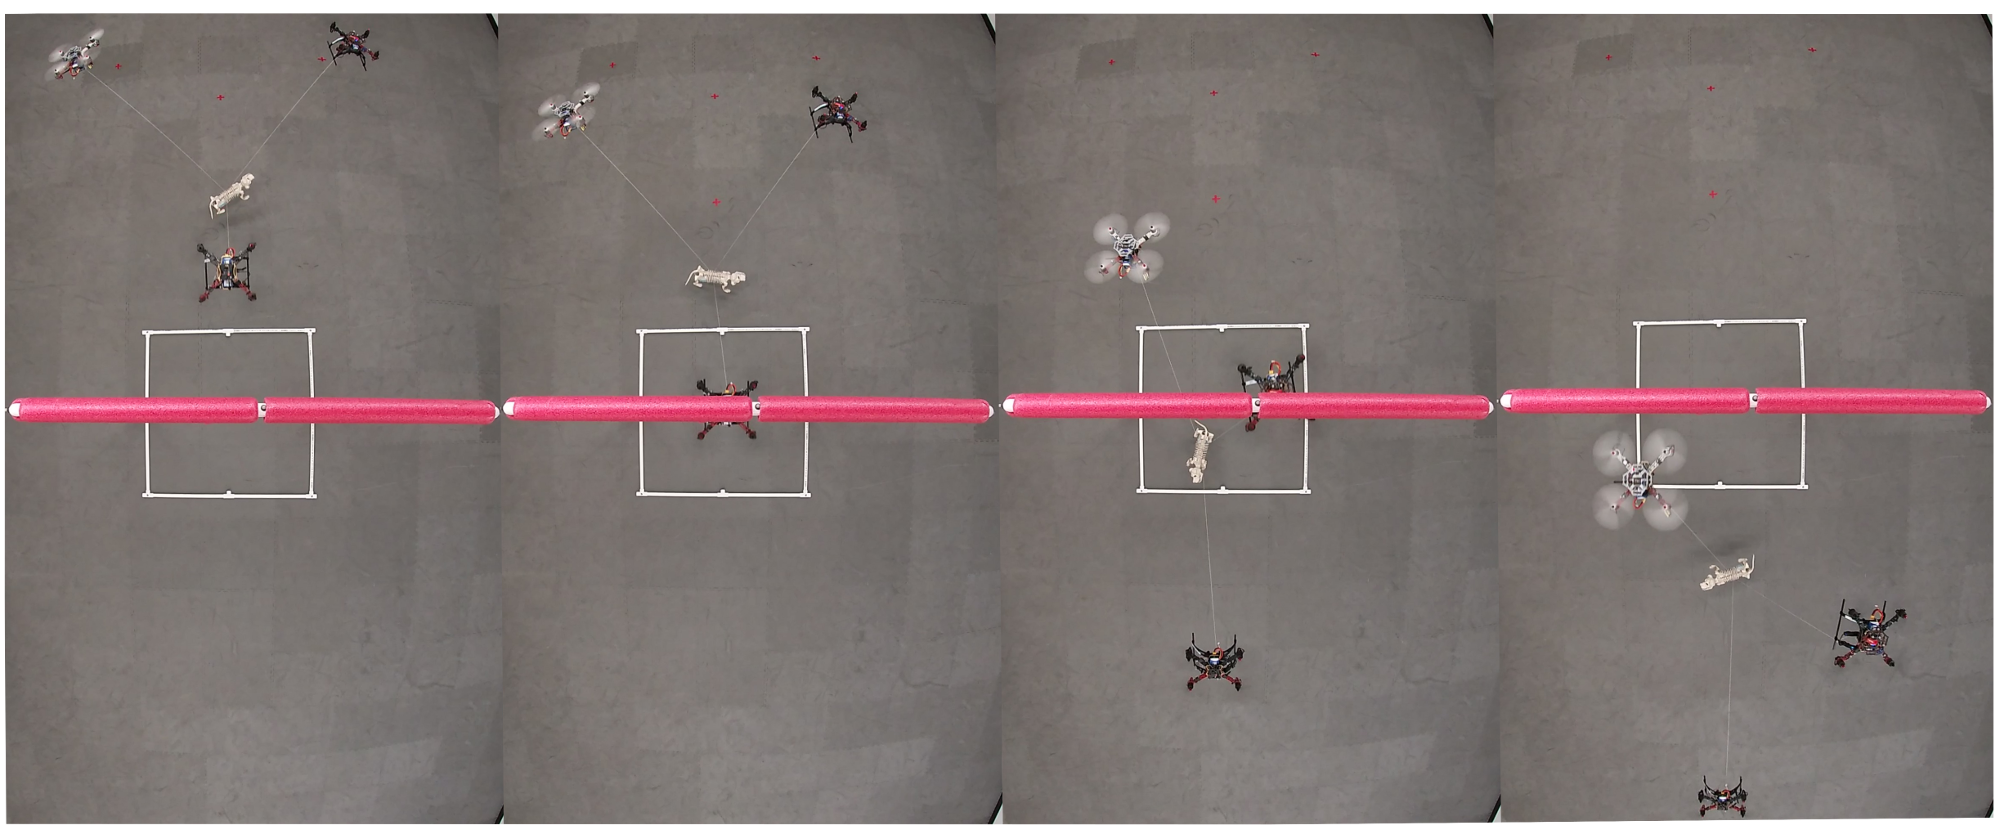
\includegraphics[width=\columnwidth,height=5.0cm]{distributed/top-side_small.png}
	\caption{Top view from hardware experiment with team of 3 quadrotors
	carrying a load through a doorway, progressing through time (left to
	right). The team reconfigures from an initial configuration that is wider
	than the doorway to a narrow configuration with the quadrotors nearly
	inline.}
	\label{topside}
\end{figure}

\section{Discussion}\label{discussion}

The current work presents a novel method for solving cable-suspended load
problems with quadrotors by posing them as nonlinear trajectory optimization
problems. By decomposing the problem and solving each sub-problem in
parallel, the algorithm is fast enough to generate new trajectories in a few
seconds (faster than the time it takes to execute them). It also scales well
to large numbers of agents, and is lightweight enough to run on
resource-constrained onboard computers that can be carried by a quadrotor.


The presented approach has many advantages, including speed, scalability, and
the ability to generate complex system-level behaviors via specification of
general constraints or the objective of the optimization problem. However,
there are also some important limitations worth noting: As with nearly all
nonlinear optimization problems, convergence is not guaranteed. The results
presented in Section \ref{hardware_results} took careful tuning of the
objective, selection of solver hyperparameters, and good initializations via
trim conditions.

Our algorithm makes no assumptions about the dynamics of the system, and
demonstrate that sub-problems can be solved in parallel across multiple
agents to achieve dramatic reductions in compute time compared to a naive
``batch'' formulation. However, our approach benefits from the inherently
sparse coupling between agents in the cable-suspended load problem, and it is
unclear how well it will generalize to other multi-agent problems with more
complicated coupling.


Several directions for future work remain: An implementation, specifically
focusing on parallelization of the batch solve and communication between
quadrotors, could likely execute faster than real-time, enable online
re-planning and model-predictive control, and be more robust than the
presented approach. Further extensions to the cable-suspended load scenario
are also possible within our approach, including lifting rigid bodies instead
of simple point masses, connecting the cables to arbitrary points on the
quadrotor, and allowing for hybrid dynamics \textit{e.g.}, slack cables.
While effective, the simplistic tracking controller used in the hardware
demonstrations can also be improved, for example, by using the LQR feedback
gains calculated by the trajectory optimization solver in the online control
loop. Finally, generalizations to a variety of other multi-agent systems with
different dynamics and constraints are possible.


\end{document}